%picfdrei,picfrecht,picfsage,picfsr,picfsd,picfss,picfar,picfad,picfas
%tabfsr,tabfsd,tabfss,tabfar,tabfad,tabfas
%subsec:rechnen
\subsection{Berechnung der Fourier-Koeffizienten} \label{subsec:rechnen}
	\begin{figure}[h]
		\begin{center}
		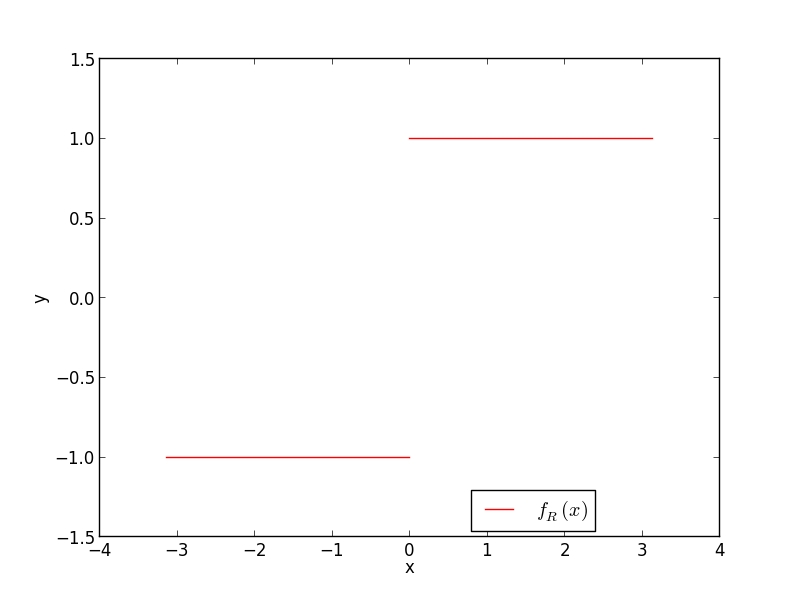
\includegraphics[scale=0.42]{picfrecht.jpg}
		\caption{Periodisch fortzusetzende Funktion $f_R$}
		\label{picfrecht}
		\end{center}	
	\end{figure} 	\begin{figure}[h]
		\begin{center}
		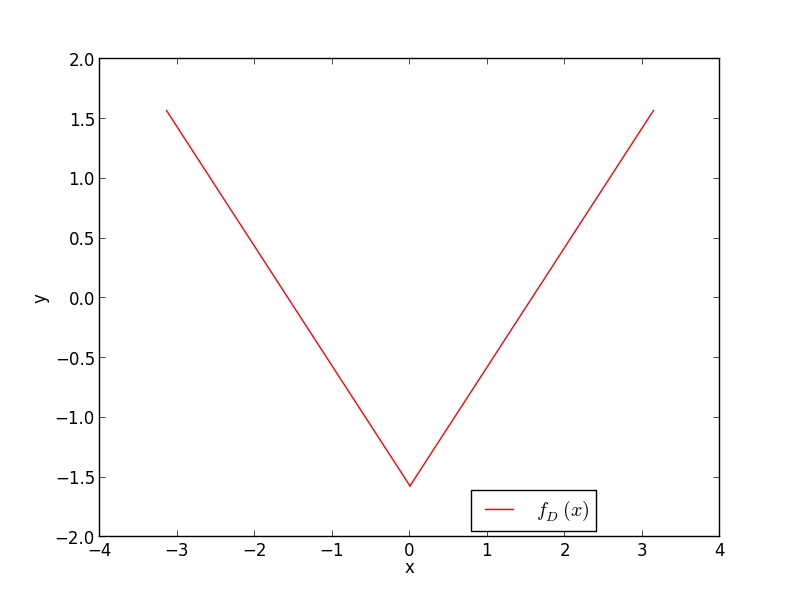
\includegraphics[scale=0.42]{picfdrei.jpg}
		\caption{Periodisch fortzusetzende Funktion $f_D$}
		\label{picfdrei}
		\end{center}	
	\end{figure} 	\begin{figure}[h]
		\begin{center}
		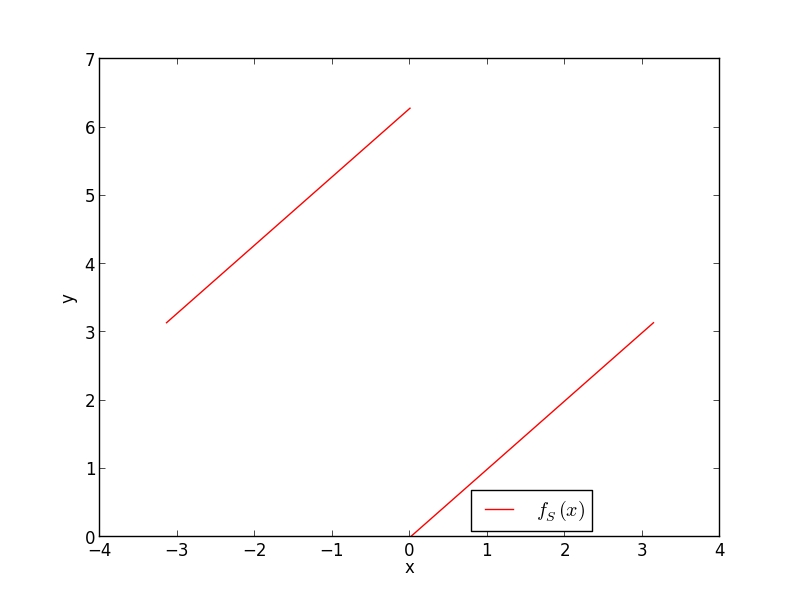
\includegraphics[scale=0.42]{picfsage.jpg}
		\caption{Periodisch fortzusetzende Funktion $f_S$}
		\label{picfsage}
		\end{center}	
	\end{figure}
Die Koeffizienten der einzelnen periodischen Funktionen berechnen sich nach den 
Gleichungen (\ref{eqfoua}) und (\ref{eqfoub}). Dabei wurde die Rechteckfunktion 
$f_R$, Abbildung (\ref{picfrecht}), als ungerade Funktion gewählt, für alle $i$ ist $a_i=0$.
Die Dreieckfunktion $f_D$, Abbildung (\ref{picfdrei}), und die Sägezahnfunktion $f_S$,
Abbildung (\ref{picfsage}), sind als gerade Funktionen definiert worden, für alle $i$ gilt
also  $b_i=0$.
\begin{align}
\text{Es gilt für die Funktionen der Definitionsbereich }&\pi \ge x > -\pi \text{ mit einer periodischen} \nonumber \\
\text{Fortsetzung von }T=2\pi \text{ .}\nonumber \\
f_R(x)&=\frac{\left| x \right|}{x}\\
f_D(x)&=\left| x \right| - \frac{\pi}{2}\\
f_S(x)&=\begin{cases}
  x + 2 \pi,  & -\pi \le x < 0\\
  x, & 0 \le x < \pi
\end{cases}\\
\text{Es ergeben sich die folgenden Fourierkoeffizienten }&\text{mit $N=1,2, \ldots$.} \nonumber \\
f_R: a_0&=0,\text{ }a_n=0, \\
b_n&=\begin{cases}
	\frac{4}{n\pi}, & n \text{ ungerade}\\
	0, & n \text{ gerade}
\end{cases}\\
f_D: a_0&=0, \text{ }b_n=0,\\
a_n&=\begin{cases}
	-\frac{4}{n^2\pi}, & n \text{ ungerade}\\
	0, & n \text{ gerade}
\end{cases}\\
f_S: a_0&=\pi, \text{ }a_n=0, \text{ }b_n=-\frac{2}{n}
\end{align}
\subsection{Fourier-Synthese}
\begin{table}[h]
	\begin{center}
		\begin{tabular}{cc}
			n&b$_\text{n}$/mV \\ \hline
			1&585,90\\
			2&0,00\\
			3&195,30\\
			4&0,00\\
			5&117,18\\
			6&0,00\\
			7&83,70\\
			8&0,00\\
			9&65,10
		\end{tabular}
		\caption{Amplituden der Fourier-Koeffizienten bei Synthese der Rechteckspannung (a$_\text{0}=\text{a}_\text{n}=0\text{ mV}$)}
		\label{tabfsr}
	\end{center}
\end{table} \begin{table}[h]
	\begin{center}
		\begin{tabular}{cc}
			n&a$_\text{n}$/mV \\ \hline
			1&585,90\\
			2&0,00\\
			3&65,10\\
			4&0,00\\
			5&23,44\\
			6&0,00\\
			7&11,96\\
			8&0,00\\
			9&7,23
		\end{tabular}
		\caption{Amplituden der Fourier-Koeffizienten bei Synthese der Dreieckspannung (a$_\text{0}=\text{b}_\text{n}=0\text{ mV}$)}
		\label{tabfsd}
	\end{center}
\end{table} \begin{table}[h]
	\begin{center}
		\begin{tabular}{cc}
			n&b$_\text{n}$/mV \\ \hline
			1&585,90\\
			2&292,90\\
			3&195,30\\
			4&146,48\\
			5&117,18\\
			6&97,65\\
			7&83,70\\
			8&73,24\\
			9&65,10
		\end{tabular}
		\caption{Amplituden der Fourier-Koeffizienten bei Synthese der Sägezahnspannung (a$_\text{0}=\text{a}_\text{n}=0\text{ mV}$)}
		\label{tabfss}
	\end{center}
\end{table} 	\begin{figure}[h]
		\begin{center}
		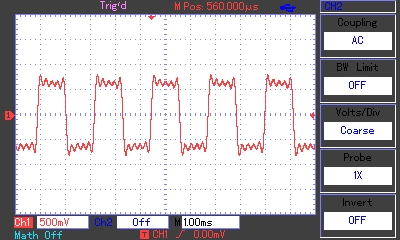
\includegraphics[scale=1.0]{picfsr.jpg}
		\caption{Fouriersynthese der Rechteckspannung}
		\label{picfsr}
		\end{center}	
	\end{figure} 	\begin{figure}[h]
		\begin{center}
		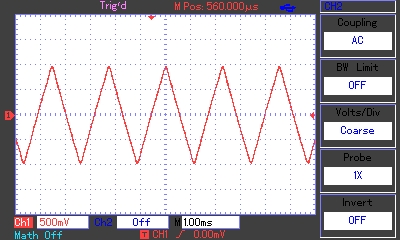
\includegraphics[scale=1.0]{picfsd.jpg}
		\caption{Fouriersynthese der Dreieckspannung}
		\label{picfsd}
		\end{center}	
	\end{figure} 	\begin{figure}[h]
		\begin{center}
		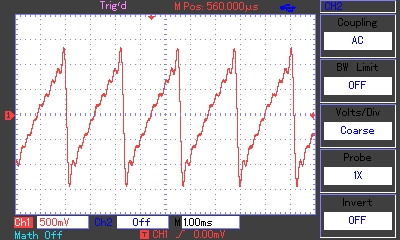
\includegraphics[scale=1.0]{picfss.jpg}
		\caption{Fourier-Synthese der Sägezahnspannung}
		\label{picfss}
		\end{center}	
	\end{figure}
Aus den Koeffizientengleichungen aus \ref{subsec:rechnen} ergeben sich die einzustellenden Amplituden
des Oberwellengenerators (Tab. \ref{tabfsr} - \ref{tabfss}). Nach der Aufsummierung der Oberwellen
ergeben sich die Graphen \ref{picfsr} bis \ref{picfss} auf dem Oszilloskop.
\FloatBarrier
\subsection{Fourier-Analyse}
\begin{table}[h]
	\begin{center}
		\begin{tabular}{cccc}
			n&b$_\text{n,mess}$/mV & b$_\text{n,theorie}$/mV & $\Delta \text{a}_\text{n}$\\ \hline
			1&7320&7320,00&0,0\%\\
			2&0&0,00&0,0\%\\
			3&2960&2440,00&21,3\%\\
			4&0&0,00&0,0\%\\
			5&1460&1464,00&0,3\%\\
			6&0&0,00&0,0\%\\
			7&1010&1045,71&3,4\%\\
			8&0&0,00&0,0\%\\
			9&952&813,33&17,0\%
		\end{tabular}
		\caption{Amplituden der Fourier-Koeffizienten bei Analyse der Rechteckspannung (a$_\text{0}=\text{a}_\text{n}=0\text{ mV}$)}
		\label{tabfar}
	\end{center}
\end{table} \begin{table}[h]
	\begin{center}
		\begin{tabular}{cccc}
			n&a$_\text{n,mess}$/mV & a$_\text{n,theorie}$/mV & $\Delta \text{a}_\text{n}$\\ \hline
			1&4760,0&4760,00&0,0\%\\
			2&0,0&0,00&0,0\%\\
			3&636,0&528,89&20,3\%\\
			4&0,0&0,00&0,0\%\\
			5&162,0&190,40&14,9\%\\
			6&0,0&0,00&0,0\%\\
			7&99,2&97,14&2,1\%\\
			8&0,0&0,00&0,0\%\\
			9&61,2&58,77&4,1\%
		\end{tabular}
		\caption{Amplituden der Fourier-Koeffizienten bei Analyse der Dreieckspannung (a$_\text{0}=\text{b}_\text{n}=0\text{ mV}$)}
		\label{tabfad}
	\end{center}
\end{table} \begin{table}[h]
	\begin{center}
		\begin{tabular}{cccc}
			n&b$_\text{n,mess}$/mV & b$_\text{n,theorie}$/mV & $\Delta \text{a}_\text{n}$\\ \hline
			1&3680&3680,00&0,0\%\\
			2&1800&1840,00&2,2\%\\
			3&1460&1226,67&19,0\%\\
			4&920&920,00&0,0\%\\
			5&716&736,00&2,7\%\\
			6&700&613,33&14,1\%\\
			7&500&525,71&4,9\%\\
			8&464&460,00&0,9\%\\
			9&464&408,89&13,5\%
		\end{tabular}
		\caption{Amplituden der Fourier-Koeffizienten bei Analyse der Sägezahnspannung (a$_\text{0}=\text{a}_\text{n}=0\text{ mV}$)}
		\label{tabfas}
	\end{center}
\end{table} 	\begin{figure}[h]
		\begin{center}
		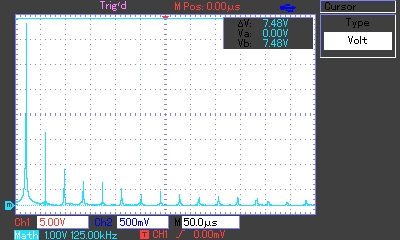
\includegraphics[scale=1.0]{picfar.jpg}
		\caption{Fourieranalyse der Rechteckspannung}
		\label{picfar}
		\end{center}	
	\end{figure} 	\begin{figure}[h]
		\begin{center}
		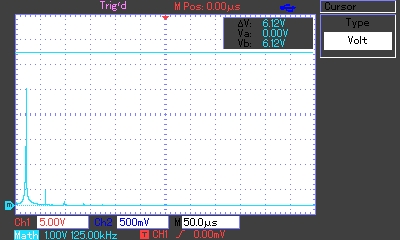
\includegraphics[scale=1.0]{picfad.jpg}
		\caption{Fourieranalyse der Dreieckspannung}
		\label{picfad}
		\end{center}	
	\end{figure} 	\begin{figure}[h]
		\begin{center}
		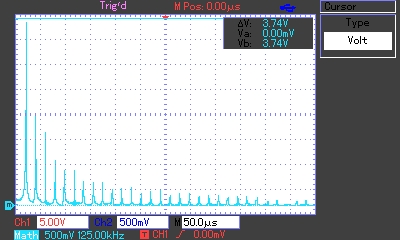
\includegraphics[scale=1.0]{picfas.jpg}
		\caption{Fourieranalyse der Sägezahnspannung}
		\label{picfas}
		\end{center}	
	\end{figure}
Die abgelesenen Amplituden in den Tabellen \ref{tabfar} bis \ref{tabfas} ergeben sich aus den Graphen
\ref{picfar} bis \ref{picfas} des Oszilloskops. Die Theoriewerte ergeben sich dabei aus der Normierung
des ersten Messwertes und der darauf aufbauenden Berechnung gemäß Gleichungen (\ref{eqfoua}) und (\ref{eqfoub}). 
